% =====================================================================
%  4. Préparation des données
% =====================================================================
\clearpage
\section{Préparation des données}
\label{sec:prep}

La préparation (notebook \notebook{02\_data\_preparation.ipynb}) transforme le
fichier brut en une table maître traçable, définit les groupes, la cohorte et
les plis, puis fournit le prétraitement qui sera appris \emph{à l'intérieur} de
chaque entraînement. Elle a d'abord été prototypée, auditée à deux reprises
(rapports 06 et 07 du dépôt), puis migrée dans ce notebook autonome ; les huit
exports migrés reproduisent exactement les exports audités.

\subsection{Deux niveaux de traitement}

Il est essentiel de distinguer deux types d'opérations :
\begin{description}[leftmargin=1em,style=nextline]
  \item[Nettoyage déterministe (global)] règles fixées \emph{a priori}, qui ne
  dépendent d'aucune statistique apprise : interpréter \texttt{N}, remplacer une
  censure par une valeur conventionnelle, isoler une unité douteuse. Elles
  peuvent être appliquées à toute la base sans fuite d'information.
  \item[Prétraitement appris (dans les plis)] opérations qui estiment des
  paramètres sur les données : moyennes et écarts-types, médianes, catégories
  connues, modèles d'imputation. Elles sont \textbf{réajustées sur chaque ensemble
  d'entraînement}, puis appliquées telles quelles à la validation correspondante.
\end{description}

\begin{intuition}
Si l'on calculait la médiane d'imputation ou la moyenne de standardisation sur
toute la base, la validation \og verrait \fg{} indirectement ses propres valeurs
à travers ces statistiques : le score serait légèrement optimiste. Ajuster ces
statistiques dans le train seulement reproduit la situation réelle, où une
nouvelle soudure arrive après l'entraînement.
\end{intuition}

\subsection{Nettoyage déterministe}
\label{subsec:nettoyage}

Le \cref{tab:nettoyage} récapitule chaque règle et sa justification. Le résultat
est une \textbf{table maître de 1\,652 lignes} (dont quatre alias marqués) et un
fichier de \textbf{provenance de 66\,080 cellules numériques} (1\,652 lignes
$\times$ 40 colonnes numériques) qui conserve, pour chaque cellule, le jeton
brut, son statut, ses bornes, l'opérateur de censure, l'annotation éventuelle,
le drapeau de revue et la valeur retenue. Aucune cible observée n'est modifiée.

\begin{table}[htbp]
\centering
\small
\caption{Règles de nettoyage déterministe et justification.}
\label{tab:nettoyage}
\begin{tabularx}{\textwidth}{@{}>{\raggedright\arraybackslash}p{3.6cm} >{\raggedright\arraybackslash}p{4.6cm} L@{}}
\toprule
Situation & Règle appliquée & Justification \\
\midrule
Lecture & 44 champs lus comme texte ; identifiant brut \texttt{raw\_row\_id} stable (0 à 1\,651) & Ne rien perdre avant d'avoir classé chaque jeton \\
\texttt{N} (non rapporté) & Valeur manquante (NaN), jamais zéro & Définition de la documentation source \\
Nombres exacts, zéros, extrêmes & Conservés & Une valeur extrême n'est pas une erreur démontrée \\
Censure \texttt{<L} sans doute d'unité & $L/2$, avec statut, opérateur et borne conservés & Approximation conventionnelle, explicitement signalée comme telle \\
Intervalle \texttt{a-b} & Milieu $(a+b)/2$, bornes conservées & 38 températures entre passes \texttt{150-200} $\to$ 175\,°C \\
Unité douteuse & NaN, sans conversion ; 322 cellules : Al 26, Ti 17, V 9, Sn/As/Sb 90 chacun & Seule la source peut confirmer l'unité (\cref{subsec:unites}) \\
Azote annoté (\texttt{tot}/\texttt{res}) & 59 annotations hors de N principal, extraction lexicale conservée & Sens total/résiduel non comparable aux autres valeurs \\
Dureté & Valeur et protocole Vickers séparés & Protocoles non regroupés automatiquement \\
Procédé & Seuls \texttt{ShMA}$\to$\texttt{MMA} et \texttt{SMA}$\to$\texttt{SA} & Synonymes documentés ; les autres procédés restent distincts \\
Courant et polarité & \texttt{N} $\to$ modalité \texttt{missing} ; aucune déduction DC/AC & Ne pas inventer une catégorie \\
Doublons hors identifiant & 4 occurrences excédentaires exclues de la cohorte et des plis ; alias conservés & Éviter qu'une même observation soit en train et en validation \\
PWHT & 13 lignes PWHT manquant conservées ; couples (0, 0) conservés & Le sens métallurgique exact du zéro n'est pas affirmé \\
\bottomrule
\end{tabularx}
\end{table}

\begin{precaution}
Les choix $L/2$ et milieu d'intervalle sont des \emph{approximations
déterministes}, pas des mesures. Ils concernent surtout des éléments absents des
schémas d'entrées retenus (Al, B, Nb, V). Pour les 16 entrées retenues, seules
47 cellules du fichier brut sont concernées : 38 intervalles de température entre passes, 7
censures de soufre et 2 de molybdène (les 59 azotes annotés étant indisponibles).
Le statut d'origine reste disponible pour toute analyse de sensibilité.
\end{precaution}

\subsection{Groupes : des séries expérimentales inférées}
\label{subsec:groupes}

Pour évaluer le transfert à de nouvelles séries, il faut d'abord les définir.
La base ne fournit pas de numéro de publication ; les groupes sont donc
\textbf{inférés des identifiants}, de manière conservatrice :
\begin{enumerate}
  \item préfixe de l'identifiant jusqu'à l'année (\ident{Evans-Ni/CMn-1990/1991-0Aaw} $\to$ \ident{Evans-Ni/CMn-1990}) ;
  \item familles explicites de rapports ou de lettres (par exemple \texttt{EvansLetter}) ;
  \item préfixe non daté, ou identifiant exact en dernier recours ;
  \item les doublons bruts relient leurs séries respectives.
\end{enumerate}
On obtient \textbf{47 groupes} sur les 1\,648 lignes dédupliquées. Les variantes
orthographiques d'auteurs (\texttt{Ga\&K}/\texttt{Gar\&K}, \texttt{Kocak}) ne sont
pas fusionnées dans le protocole actif. Ces groupes sont des \emph{séries
inférées}, pas des publications vérifiées : une série peut regrouper plusieurs
conditions de soudage (\cref{subsec:decoupages}).

\subsection{Cohorte de modélisation}
\label{subsec:cohorte}

Ni, Cr et Mo sont absents dans plus de la moitié des lignes ; d'autres entrées
le sont plus rarement. Nous définissons une cohorte qui limite le nombre
d'entrées à reconstruire tout en conservant un maximum de séries :

\begin{decision}
\textbf{Cohorte principale} : lignes non dupliquées ayant \textbf{au plus deux
entrées numériques indisponibles parmi les 13 entrées du schéma A1\_13}
(\cref{tab:schemas}). Elle compte \textbf{1\,555 lignes réparties en 44 groupes} ;
trois séries (\texttt{Cunh-1982}, \texttt{EvHtIp1979}, \texttt{Natsume-1990})
sortent entièrement. Les seuils alternatifs $\leq 1$ et $\leq 3$ donneraient
1\,087 et 1\,603 lignes, 34 et 46 groupes, 501 et 748 labels de \YS{} : le
seuil 2 est un compromis d'ingénierie entre couverture et quantité d'imputation,
pas une garantie de fiabilité.
\end{decision}

\begin{figure}[htbp]
\centering
\begin{tikzpicture}[
  bloc/.style={rectangle, rounded corners=2pt, draw=csbordeaux, line width=0.7pt,
               fill=csgrisclair, align=center, minimum height=1.05cm, font=\footnotesize},
  cible/.style={rectangle, rounded corners=2pt, draw=csgris, line width=0.6pt,
               fill=white, align=center, minimum height=0.95cm, text width=2.55cm, font=\scriptsize},
  fleche/.style={-{Stealth[length=2mm]}, line width=0.8pt, color=csgris},
  lab/.style={font=\scriptsize\itshape, color=encre2, align=left}]
  \node[bloc, text width=3.1cm] (brut) {\textbf{1\,652 lignes brutes}\\ 44 colonnes};
  \node[bloc, text width=3.1cm, right=1.9cm of brut] (dedup) {\textbf{1\,648 lignes}\\ dédupliquées, 47 groupes};
  \node[bloc, text width=3.4cm, right=1.9cm of dedup] (coh) {\textbf{1\,555 lignes, 44 groupes}\\ cohorte $\leq 2$ absences sur A1\_13};
  \draw[fleche] (brut) -- node[above, lab] {$-4$ alias} (dedup);
  \draw[fleche] (dedup) -- node[above, lab] {$-93$ lignes} (coh);
  \node[cible, below=1.25cm of brut.south west, anchor=north west] (ys) {\textbf{\YS} : 706 labels\\ 40 groupes ; pool 849};
  \node[cible, right=0.35cm of ys] (uts) {\textbf{\UTS} : 677 labels\\ 39 groupes ; pool 878};
  \node[cible, right=0.35cm of uts] (el) {\textbf{Allongement} : 631\\ 34 groupes ; pool 924};
  \node[cible, right=0.35cm of el] (ch) {\textbf{\charpy} : 861\\ 24 groupes ; pool 0};
  \draw[fleche] (coh.south) -- ++(0,-0.45) -| (ys.north);
  \draw[fleche] (coh.south) -- ++(0,-0.45) -| (uts.north);
  \draw[fleche] (coh.south) -- ++(0,-0.45) -| (el.north);
  \draw[fleche] (coh.south) -- ++(0,-0.45) -| (ch.north);
\end{tikzpicture}
\caption{Du fichier brut aux populations de modélisation. Chaque cible utilise les
lignes de la cohorte qui la renseignent ; les autres lignes de la cohorte forment
son pool non étiqueté (vide pour Charpy, faute de température d'essai connue sans énergie).}
\label{fig:entonnoir}
\end{figure}

Dans la cohorte, \textbf{607 lignes} ont au moins une entrée absente parmi les
13, soit \textbf{1\,075 cellules}. La table maître conserve ces NaN : aucune
table globalement imputée n'est utilisée par les modèles. Parmi les lignes
dédupliquées, 105 n'ont aucune des cinq sorties traction/Charpy (99 dans la
cohorte) ; elles sont conservées comme exemples non étiquetés.

\subsection{Schémas d'entrées}
\label{subsec:schemas}

Trois schémas emboîtés ont été définis et comparés (\cref{tab:schemas}). Le
schéma de départ A1\_13 privilégiait des entrées bien renseignées ; l'extension
A1b\_16 ajoute Ni, Cr et Mo, éléments d'alliage métallurgiquement importants
mais souvent absents (\cref{fig:absences_cohorte}). Passer de 13 à 16 entrées
\textbf{ajoute des colonnes, pas des lignes} : la cohorte n'est pas refiltrée.

\begin{table}[htbp]
\centering
\small
\caption{Schémas d'entrées numériques ; le procédé catégoriel est ajouté à chacun.}
\label{tab:schemas}
\begin{tabularx}{\textwidth}{@{}l c L@{}}
\toprule
Schéma & Entrées & Variables \\
\midrule
A0\_11  & 11 & C, Si, Mn, S, P, courant, tension, apport thermique, température entre passes, température et durée PWHT \\
A1\_13  & 13 & A0\_11 $+$ oxygène et azote \\
A1b\_16 & 16 & A1\_13 $+$ nickel, chrome et molybdène \\
\bottomrule
\end{tabularx}
\end{table}

\begin{figure}[htbp]
\centering
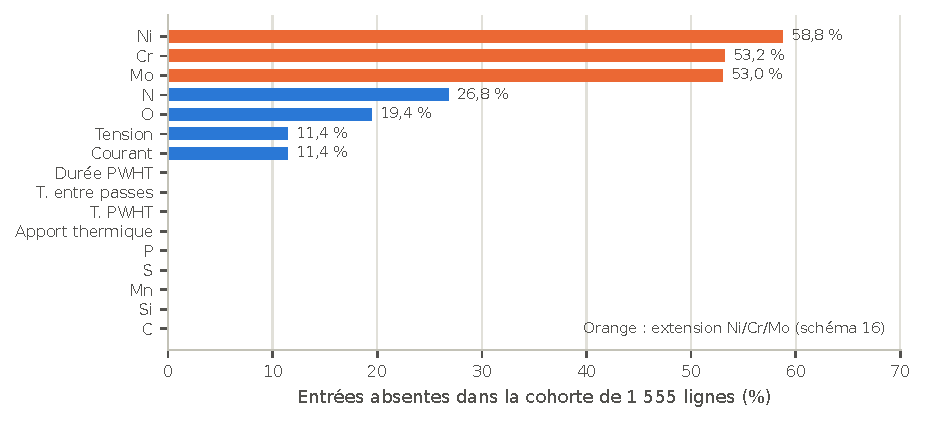
\includegraphics[width=0.95\textwidth]{prep_absences_cohorte}
\caption{Part d'entrées absentes dans la cohorte de 1\,555 lignes pour les
16 entrées numériques. Ni, Cr et Mo manquent dans plus de la moitié des lignes.}
\label{fig:absences_cohorte}
\end{figure}

\subsection{Normalisation : pourquoi standardiser ?}
\label{subsec:standardisation}

Chaque entrée numérique est standardisée avec la moyenne $\mu_j$ et
l'écart-type $\sigma_j$ calculés sur les valeurs \emph{observées} du train :
\begin{equation}
  z_{ij} = \frac{x_{ij} - \mu_j^{\text{train}}}{\sigma_j^{\text{train}}}.
\end{equation}
Cette étape est indispensable pour les méthodes fondées sur des distances ou des
normes : le $k$NN, la SVR à noyau RBF (dont le noyau
$\exp(-\gamma\lVert\bm{x}-\bm{x}'\rVert^2)$ dépend des échelles) et la régression
Ridge (dont la pénalité $\lambda\lVert\bm{\beta}\rVert^2$ traite tous les
coefficients de la même manière). Elle est sans effet sur les partitions d'une
forêt aléatoire, mais elle est conservée pour que toutes les familles partagent
exactement la même représentation. Le procédé est encodé en \emph{one-hot} sur
les catégories vues dans le train ; une catégorie inconnue devient un vecteur nul.
Pour la SVR uniquement, la cible $y$ est aussi standardisée dans le train, puis
les prédictions sont remises dans leur unité physique.

\subsection{Imputation des entrées manquantes}
\label{subsec:imputation}

Deux méthodes d'imputation ont été mises en œuvre, toutes deux \textbf{ajustées
dans chaque train} et appliquées aux seules \emph{entrées} :
\begin{description}[leftmargin=1em,style=nextline]
  \item[Médiane] chaque valeur manquante reçoit la médiane de la colonne dans le
  train. Simple et stable, elle ignore les relations entre variables.
  \item[Itérative] (\emph{chained equations})~\cite{vanbuuren_2011} chaque
  colonne incomplète est régressée sur les autres par une régression bayésienne
  ridge (\texttt{IterativeImputer} + \texttt{BayesianRidge}), en alternant
  jusqu'à convergence : initialisation médiane, ordre ascendant, au plus 100
  itérations, tolérance $10^{-3}$, graine 42, bornes non négatives.
\end{description}
Après imputation, un PWHT reconstruit est projeté sur un couple
(température, durée) \emph{réellement observé} dans le train, au plus proche en
distance standardisée et compatible avec une composante observée. Toute situation
anormale --- colonne entièrement absente du train, absence de couple compatible,
non-convergence de l'imputation itérative --- déclenche une \textbf{erreur
explicite}, sans repli silencieux. Les cibles ne sont jamais transmises à
l'imputeur.

\paragraph{Pourquoi l'itérative au départ ?} Une étude historique de
reconstruction (5 octobre) masquait artificiellement 10, 20 ou 40\,\% de valeurs
exactes et comparait les méthodes sur des plis par séries (\cref{tab:reconstruction}).
Sur 11 entrées, l'itérative reconstruisait le mieux ; sur une extension à
22 entrées, elle ne convergeait dans aucun pli.

\begin{table}[htbp]
\centering
\small
\caption{Étude historique de reconstruction de valeurs masquées (3 plis par
séries, graines 42/43). MAE normalisée par l'écart interquartile du train ; plus
bas est meilleur.}
\label{tab:reconstruction}
\begin{tabular}{@{}llrrr@{}}
\toprule
Entrées & Méthode & MAE normalisée & $\Delta$ corrélations & Plis convergés \\
\midrule
11 (noyau)    & Médiane              & 1,697 & 0,084 & 3/3 \\
11 (noyau)    & Médiane par procédé  & 1,254 & 0,069 & 3/3 \\
11 (noyau)    & Itérative            & \meilleur{0,853} & \meilleur{0,066} & 3/3 \\
22 (étendu)   & Médiane              & 2,253 & 0,106 & 3/3 \\
22 (étendu)   & Médiane par procédé  & 2,060 & 0,106 & 3/3 \\
22 (étendu)   & Itérative            & 2,009 & 0,159 & 0/3 \\
\bottomrule
\end{tabular}
\end{table}

Un contrôle à paramètres fixes, sur le schéma A1\_13 et les plis groupés, a
ensuite comparé les deux imputations sous une forêt aléatoire (300 arbres,
feuille minimale 2, graine 42). Les 15 ajustements itératifs convergeaient en
4 à 7 itérations, et l'itérative n'était pas uniformément meilleure
(\cref{tab:controle_imputation}).

\begin{table}[htbp]
\centering
\small
\caption{Contrôle d'imputation à paramètres fixes, schéma 13, validation groupée
(MAE moyenne des cinq plis externes).}
\label{tab:controle_imputation}
\begin{tabular}{@{}lrrrr@{}}
\toprule
Cible & Baseline médiane & RF / médiane & RF / itérative & \Rdeux{} RF / itérative \\
\midrule
\YS{} (MPa)               & 70,45 & \meilleur{65,39} & 66,13 & 0,077 \\
\UTS{} (MPa)              & 72,66 & 58,10 & \meilleur{56,71} & 0,190 \\
Allongement (points de \%) & 4,09 & 3,70 & \meilleur{3,55} & 0,114 \\
\bottomrule
\end{tabular}
\end{table}

\begin{decision}
Le premier benchmark supervisé utilise \textbf{A1\_13 avec imputation
itérative}, justifiée par l'étude de reconstruction. Les diagnostics
(\cref{subsec:sensibilites}) montreront ensuite que l'itérative \textbf{ne converge
pas} dans 11 contextes sur 16 entrées, alors que la médiane reste stable et que
l'ajout de Ni/Cr/Mo améliore nettement \YS{} et \UTS. La configuration de travail
devient alors \textbf{A1b\_16 avec imputation médiane}. Ce choix est
rétrospectif : il a été fait après observation des scores sur ces mêmes données.
\end{decision}

\subsection{Le prétraitement complet dans une pipeline}

Toutes les étapes apprises sont encapsulées dans une \texttt{Pipeline} de
scikit-learn~\cite{pedregosa_2011} : la classe \texttt{FoldPreprocessor}, définie
dans le notebook 02, est suivie de l'estimateur. La \cref{fig:pipeline} illustre son
fonctionnement : la même pipeline est ajustée sur le train, puis appliquée
sans réajustement à la validation et, pour COREG, au pool non étiqueté.

\begin{figure}[htbp]
\centering
\begin{tikzpicture}[
  etape/.style={rectangle, rounded corners=2pt, draw=csbordeaux, line width=0.6pt,
                fill=csgrisclair, align=center, text width=2.05cm, minimum height=1.15cm,
                font=\scriptsize},
  data/.style={rectangle, draw=csgris, line width=0.6pt, fill=white, align=center,
               text width=1.8cm, minimum height=0.85cm, font=\scriptsize},
  fit_/.style={-{Stealth[length=1.8mm]}, line width=0.75pt, color=csbordeaux},
  app/.style={-{Stealth[length=1.8mm]}, line width=0.75pt, color=bleuviz, dashed},
  node distance=0.32cm]
  \node[data] (xtr) {Train\\ $(X, y)$ étiqueté};
  \node[etape, right=0.45cm of xtr] (s1) {Moyenne/écart-type\\ des valeurs observées};
  \node[etape, right=of s1] (s2) {One-hot du procédé\\ (catégories du train)};
  \node[etape, right=of s2] (s3) {Imputation\\ médiane ou itérative};
  \node[etape, right=of s3] (s4) {Garde PWHT\\ (couples du train)};
  \node[etape, right=of s4, fill=white, draw=csgris] (m) {Modèle\\ (Ridge, SVR,\\ RF, $k$NN)};
  \node[data, below=1.15cm of xtr] (xva) {Validation $X$\\ ou pool $U$};
  \node[data, below=1.15cm of m] (pred) {Prédictions\\ $\hat{y}$ $\to$ métriques};
  \draw[fit_] (xtr) -- (s1);
  \draw[fit_] (s1) -- (s2);
  \draw[fit_] (s2) -- (s3);
  \draw[fit_] (s3) -- (s4);
  \draw[fit_] (s4) -- (m);
  \draw[app] (xva) -- node[below, font=\scriptsize, color=bleuviz!80!black] {transformations figées (aucun réajustement)} (pred);
  \draw[app] (m) -- (pred);
  \node[font=\scriptsize, color=csbordeaux, above=0.08cm of s3] {ajustement (fit) sur le train uniquement};
\end{tikzpicture}
\caption{Pipeline de prétraitement et de modélisation. Les flèches pleines
indiquent les paramètres appris sur le train ; la flèche pointillée, l'application
de ces paramètres figés à la validation (ou au pool non étiqueté).}
\label{fig:pipeline}
\end{figure}

\begin{aretenir}
\begin{itemize}[leftmargin=1.2em]
  \item Nettoyage \textbf{déterministe et traçable} (66\,080 cellules documentées) ; brut inchangé ; aucune cible modifiée ou imputée.
  \item \textbf{47 groupes} de séries inférées ; cohorte de \textbf{1\,555 lignes / 44 groupes} avec au plus deux entrées manquantes sur 13.
  \item Standardisation, encodage et imputation sont \textbf{appris dans chaque train} via une pipeline unique.
  \item Configuration initiale 13/itérative, puis configuration de travail \textbf{16/médiane} après diagnostic.
\end{itemize}
\end{aretenir}
